\documentclass{standalone}
\usepackage{tikz}
\begin{document}
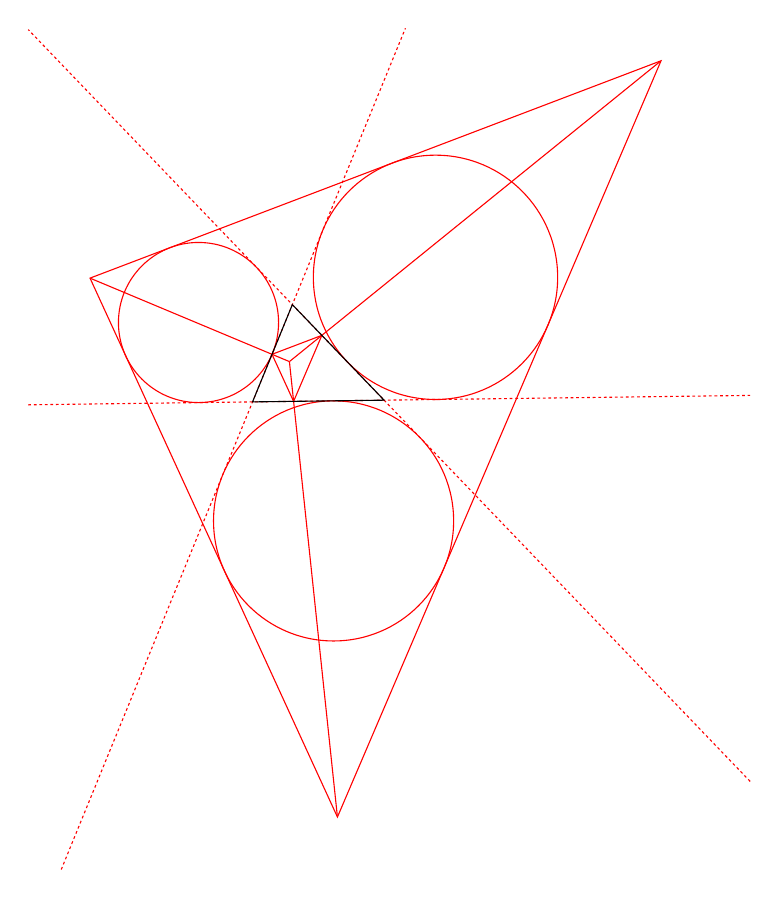
\begin{tikzpicture}[x=1pt,y=1pt]
\draw[red] (145.17,-88.01) circle (44.14);
\draw[red] (108.34,-176.03) circle (43.38);
\draw[red] (59.53,-104.34) circle (28.93);
\draw[red, dash pattern=on 1pt] (9.93,-302.00) -- (134.30,2.00);
\draw[red, dash pattern=on 1pt] (258.86,-270.15) -- (-2.00,1.51);
\draw[red, dash pattern=on 1pt] (-2.00,-134.08) -- (258.86,-130.68);
\draw[red] (92.38,-118.46) -- (20.70,-88.46);
\draw[red] (92.38,-118.46) -- (109.66,-282.36);
\draw[red] (92.38,-118.46) -- (226.18,-10.15);
\draw[red] (109.73,-283.03) -- (226.67,-9.76) -- (20.33,-88.30) -- cycle;
\draw[red] (93.89,-132.83) -- (104.10,-108.98) -- (86.09,-115.83) -- cycle;
\draw (79.06,-133.02) -- (126.59,-132.40) -- (93.44,-97.88) -- cycle;
\end{tikzpicture}
\end{document}
